\section{实验}

\subsection{实验准备}
本次实验使用高分一号影像和哨兵二号影像作为原始数据, 经过预处理, 裁剪, 筛选, 直方图匹配后, 得到遥感超分影像数据集. 选择1200对作为训练数据, 5对作为测试数据, 进行训练. 使用的模型为\href{https://github.com/RaoUmer/SRResCGAN}{srrescgan}, 由于还未透彻理解GAN, 暂时不讲具体的模型结构. 

\subsection{训练过程}
total loss从一开始的100左右降到90左右, 共419个epoch. 训练结果不太理想, 需要重新调整学习率. 使用Adam优化器, $\beta_{1}=0.9$, $\beta_2={0.999}$

\subsection{实验结果分析}
实验结果使用传统的Bicubic采样方式进行上采样, 超分模型得到结果和其真值进行对比. 

\begin{figure}[!htbp]
    \centering
    \subfloat[BC]{\label{fig:0101a}
    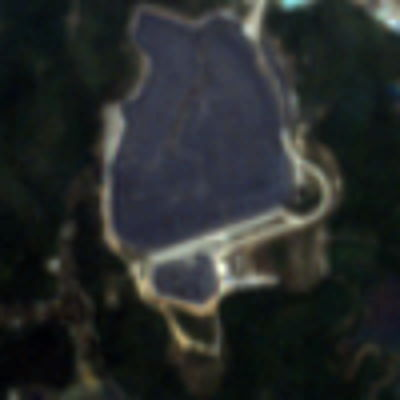
\includegraphics[height=10em]{pic/img1_LR_bicubic.jpg}}
    \quad
    \subfloat[SR]{\label{fig:0101b}
    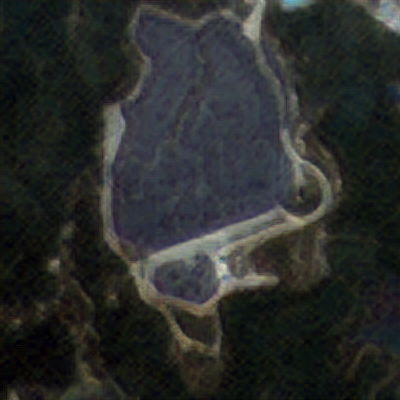
\includegraphics[height=10em]{pic/img1_SR.jpg}}
    \quad
    \subfloat[GT]{\label{fig:0101c}
    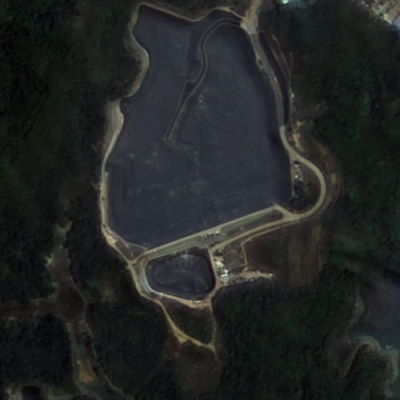
\includegraphics[height=10em]{pic/img1_GT.jpg}}
    \caption{result01}
    \label{fig:0101}
\end{figure}

\begin{figure}[!htbp]
    \centering
    \subfloat[BC]{\label{fig:0102a}
    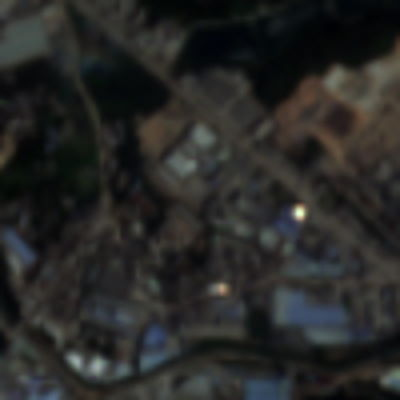
\includegraphics[height=10em]{pic/img2_LR_bicubic.jpg}}
    \quad
    \subfloat[SR]{\label{fig:0102b}
    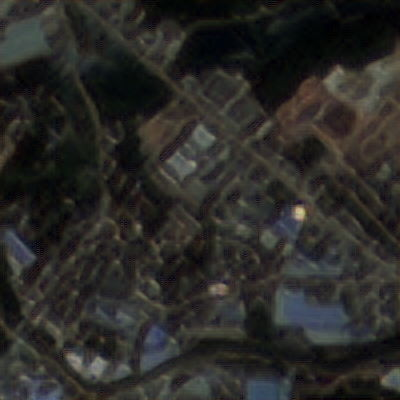
\includegraphics[height=10em]{pic/img2_SR.jpg}}
    \quad
    \subfloat[GT]{\label{fig:0102c}
    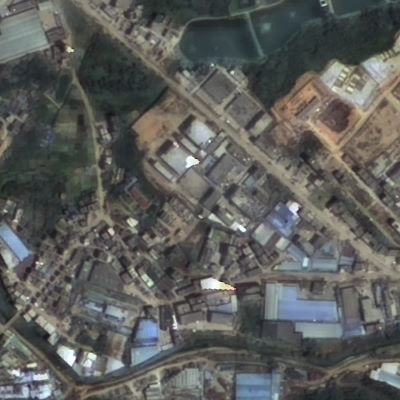
\includegraphics[height=10em]{pic/img2_GT.jpg}}
    \caption{result02}
    \label{fig:0102}
\end{figure}

\begin{figure}[!htbp]
    \centering
    \subfloat[BC]{\label{fig:0103a}
    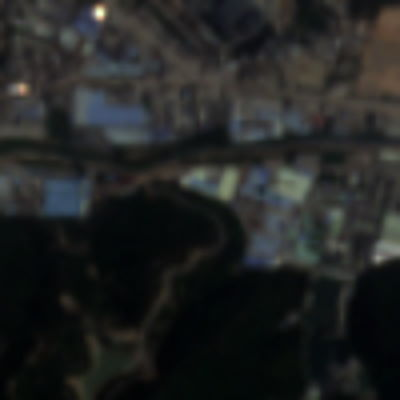
\includegraphics[height=10em]{pic/img3_LR_bicubic.jpg}}
    \quad
    \subfloat[SR]{\label{fig:0103b}
    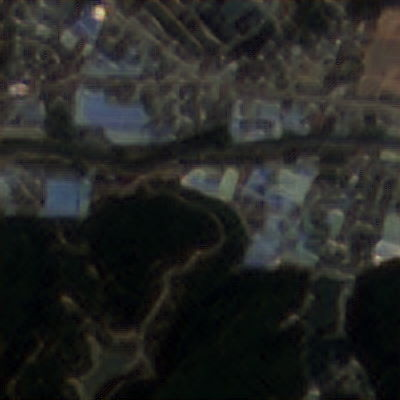
\includegraphics[height=10em]{pic/img3_SR.jpg}}
    \quad
    \subfloat[GT]{\label{fig:0103c}
    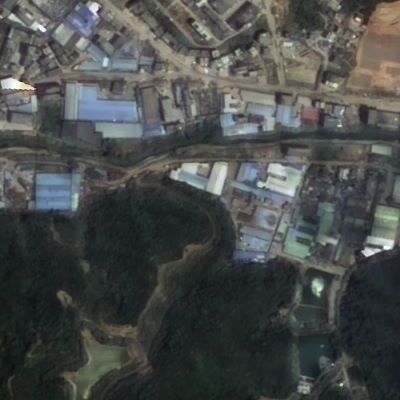
\includegraphics[height=10em]{pic/img3_GT.jpg}}
    \caption{result03}
    \label{fig:0103}
\end{figure}

\begin{figure}[!htbp]
    \centering
    \subfloat[BC]{\label{fig:0104a}
    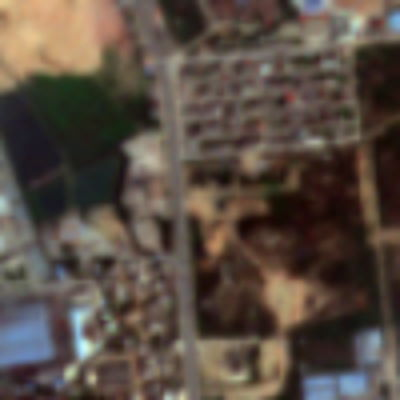
\includegraphics[height=10em]{pic/img4_LR_bicubic.jpg}}
    \quad
    \subfloat[SR]{\label{fig:0104b}
    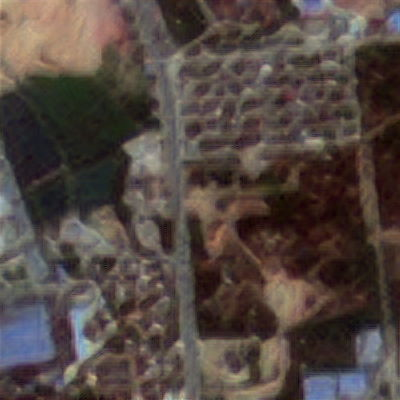
\includegraphics[height=10em]{pic/img4_SR.jpg}}
    \quad
    \subfloat[GT]{\label{fig:0104c}
    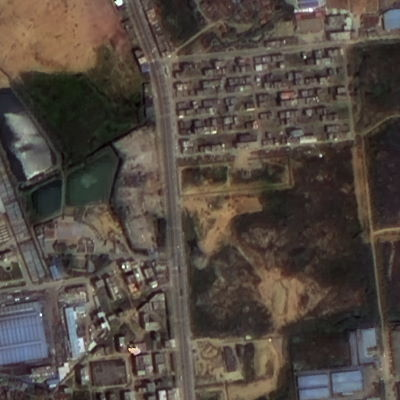
\includegraphics[height=10em]{pic/img4_GT.jpg}}
    \caption{result04}
    \label{fig:0104}
\end{figure}

\begin{figure}[!htbp]
    \centering
    \subfloat[BC]{\label{fig:0105a}
    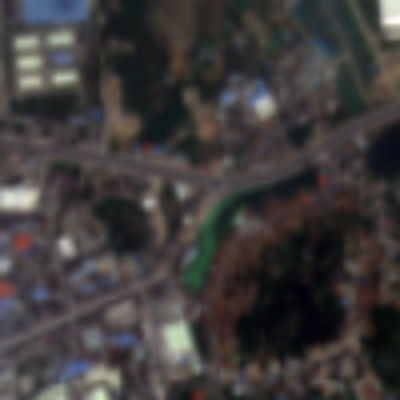
\includegraphics[height=10em]{pic/img5_LR_bicubic.jpg}}
    \quad
    \subfloat[SR]{\label{fig:0105b}
    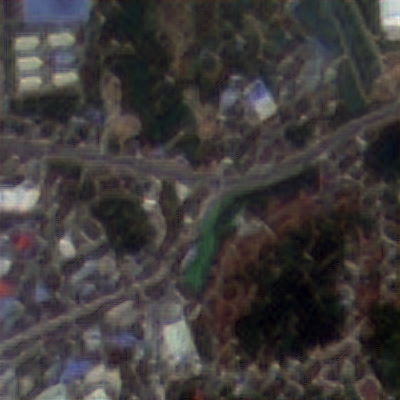
\includegraphics[height=10em]{pic/img5_SR.jpg}}
    \quad
    \subfloat[GT]{\label{fig:0105c}
    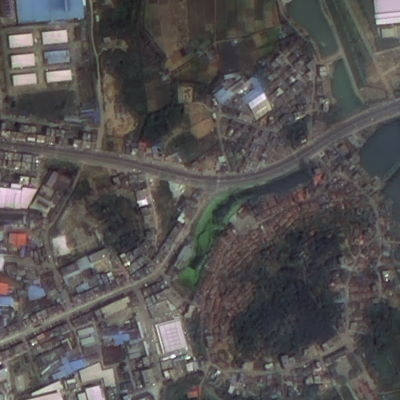
\includegraphics[height=10em]{pic/img5_GT.jpg}}
    \caption{result05}
    \label{fig:0105}
\end{figure}

\begin{table}[!htbp]
    \centering
    \begin{tabular}{c|p{3cm}|p{3cm}}
        \hline
                 & Bicubic & SRrescgan     \\ \hline
        PNSR01 & 21.97dB   & 22.73dB$\uparrow$    \\ \hline
        SSIM01 & 0.7001   & 0.6787$\downarrow$     \\ \hline
        PNSR02 & 12.68dB   & 12.81dB$\uparrow$     \\ \hline
        SSIM02 & 0.2436   & 0.2671$\uparrow$     \\ \hline
        PNSR03 & 14.65dB   & 14.77dB$\uparrow$     \\ \hline
        SSIM03 & 0.2973   & 0.3302$\uparrow$    \\ \hline
        PNSR04 & 18.87dB   & 19.55dB$\uparrow$     \\ \hline
        SSIM04 & 0.4163   & 0.3960$\downarrow$     \\ \hline
        PNSR05 & 18.06   & 18.35dB$\uparrow$     \\ \hline
        SSIM05 & 0.4064   & 0.3906$\downarrow$     \\ \hline

    \end{tabular}
    \caption{定量结果}
\end{table}


% \begin{figure}[!htbp]
%     \centering
%     \subfloat[BC]{\label{fig:0105a}
%     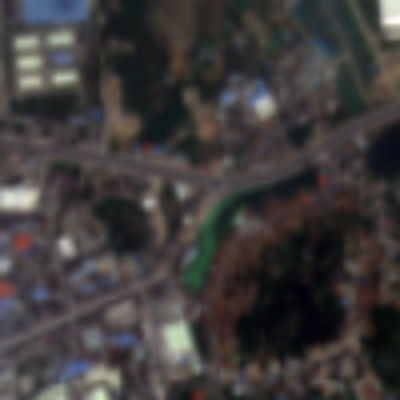
\includegraphics[height=10em]{pic/img5_LR_bicubic.jpg}}
%     \quad
%     \subfloat[SR]{\label{fig:0105b}
%     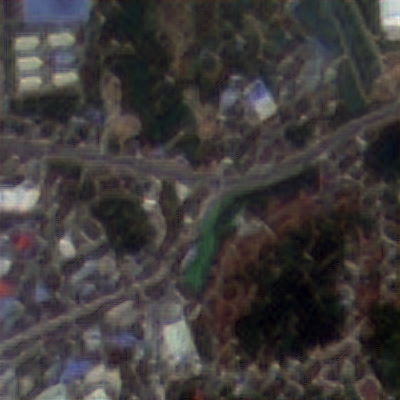
\includegraphics[height=10em]{pic/img5_SR.jpg}}
%     \quad
%     \subfloat[GT]{\label{fig:0105c}
%     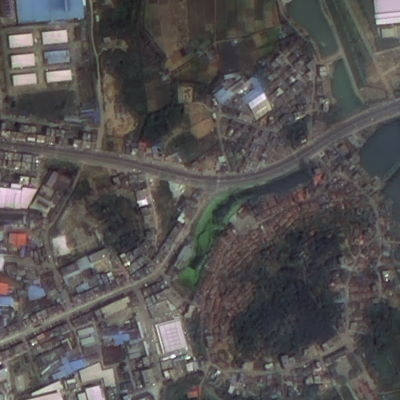
\includegraphics[height=10em]{pic/img5_GT.jpg}}
%     \caption{result05}
%     \label{fig:0105}
% \end{figure}